\chapter{Carry Scheduling and Universal Single-Prime Rigidity}\label{ch:schedule}

Theorem~\ref{thm:odometer} describes a persistent orbit in its eventual regime as a family of independent counters, one per active prime. This chapter proves that the family has exactly one member. Whatever the modulus \(g\) and whatever the seed, a single prime carries forever and every other prime is frozen. This is the rigidity of the volume's title, and it has three consequences: the scaling factor is a prime power (Theorem~\ref{thm:rho}), the reach counting function is logarithmic for every orbit (Corollary~\ref{cor:logreach}), and the two natural clocks of two saturated primes have coprime periods (Theorem~\ref{thm:coprime}).

\section{The carry scheduler}

Notation as in Chapter~\ref{ch:gamma}: a persistent orbit with \(G=g\), exponent state \(E=(e_p)\), \(o_p=\ord_g(p)\), \(w=\gamma+1\). By Theorem~\ref{thm:closure} the orbit is eventually class-periodic. A prime is \emph{active} if its exponent is unbounded and \emph{inert} otherwise. After a finite time only active primes change their exponent, every active prime is saturated (\(e_p\ge o_p-1\)), and (Theorems~\ref{thm:carrycomp},~\ref{thm:primepower}) every carry is complete and a prime power \(p^j\), with \(\gamma=1\) immediately before it and \(w=p^{2j}\).

For a state \(E\) and a prime \(p\nmid g\) put \(e=e_p\) (0 if \(p\nmid L\)) and define the \emph{pending carry}
\[
j_p(E)=\min\{j\ge1:\ p^{e+j}a\equiv1\ (\mathrm{mod}\ g)\text{ for some }a\in\mathcal A_{-p}(E)\},\qquad c_p(E)=p^{j_p(E)},
\]
where \(\mathcal A_{-p}(E)\) is the set of residues of divisors of \(\prod_{q\ne p}q^{e_q}\) (\(j_p=\infty\) if no \(j\le o_p\) works).

\begin{theorem}[The carry scheduler]\rec{F.T59}\scope{C}\label{thm:scheduler}
At a reset state (\(\gamma=1\)) of the eventual regime the next carry is carried out by the prime \(p\) with the smallest pending carry \(c_p(E)\); there are no ties. Its exponent increases by \(j_p\), no other exponent changes, the \(\gamma\)-cycle is \(1,2,\dots,c_p^2-1\), and the next reset occurs after \(c_p^2-1\) steps. The orbit stays persistent iff \(c_p^2<g\) (\(g\) odd; \(c_p^2<4g\) for \(g\) even). Moreover:
\begin{enumerate}[label=(\alph*),nosep]
\item for an active \(p\), \(c_p\) is a function of \(e_p\bmod o_p\) alone: \(c_p=p^{\mathrm{gap}_p(e_p)}\) with \(\mathrm{gap}_p(e)=\min\{j\ge1:(e+j)\bmod o_p\in\Abs_p\}\);
\item for an inert prime \(c_p\) is constant;
\item after \(p\) fires, \(e_p\bmod o_p\in\Abs_p\), and each further firing moves \(e_p\bmod o_p\) to the next element of \(\Abs_p\) in the cyclic order of \(\Z/o_p\), so \(p\) visits every element of \(\Abs_p\) cyclically.
\end{enumerate}
\end{theorem}
\begin{proof}
By Theorem~\ref{thm:carrycomp} the next carry from \(\gamma=1\) is the smallest \(M\) available at \(w=M^2\). By Theorem~\ref{thm:absorb} a new part \(M(d)\) is available iff \(M(d)^2\mid w\). In the eventual regime a composite \(M(d)\) involves \(\ge2\) primes whose exponents change, hence active, hence saturated; by the argument of Theorem~\ref{thm:primepower} such an \(M\) is not minimal. So the minimal available \(M\) is a prime power \(p^j\), and \(p^j\) is available iff \(p^{e+j}a\equiv1\) for some \(a\in\mathcal A_{-p}\), i.e. iff \(j\ge j_p\); the smallest available \(M\) is \(\min_pp^{j_p}\). Ties are impossible: \(p^a=q^b\) with \(a,b\ge1\) has no solution for \(p\ne q\). The persistence window is Theorem~\ref{thm:window}(c). For (a): for a saturated prime, the residue set of \(\langle q\rangle\) does not depend on \(e_q\), and for an inert prime it is constant; so \(c_p\) depends on \(E\) only through \(e_p\) and the residues of the other primes, which are constant in time. Hence \(c_p\) depends on \(e_p\bmod o_p\) alone. (b) is the same observation. (c): after \(p\) fires, \(p^{e_p}a\equiv1\) for some \(a\), so \(e_p\bmod o_p\in\Abs_p\); the next firing advances to the next element by definition of \(\mathrm{gap}_p\).
\end{proof}

\section{Single-prime dominance}

\begin{theorem}[Single-prime dominance]\rec{F.T60}\scope{C}\label{thm:dominance}
In the eventual regime of every persistent orbit (every \(g\), every seed) exactly one prime is active. Equivalently: there are no \(x_0\) and no primes \(p\ne q\) such that \(p\) and \(q\) both carry infinitely often. The same holds for every abstract system of cyclic odometers \((\Z/s_i,C_i,p_i)\), \(s_i\ge1\), \(C_i\ne\emptyset\), with the minimum-pending-carry rule.
\end{theorem}
\begin{proof}
\emph{At least one prime is active.} Otherwise \(L\) is eventually constant, and \(\gamma_n\le2M\) eventually (Theorem~\ref{thm:T47}) would make \(x_n\) bounded, while \(x_{n+1}>x_n\).

\emph{At most one.} For an active prime \(r\) let
\[
m_r=\max\{r^{\mathrm{gap}_r(k)}:k\in\Abs_r\}
\]
be its \emph{worst-case pending carry}. Since every \(k\bmod o_r\) lies in a gap of \(\Abs_r\), we have \(c_r\le m_r\) at all times after \(r\) has fired once (Theorem~\ref{thm:scheduler}(a)). Suppose two distinct primes are active. Distinct primes never have equal powers, so the numbers \(m_r\) (\(r\) active) are pairwise distinct; let \(p\) be the active prime with the largest \(m_r\), and \(q\) any other active prime, so \(m_q<m_p\).

Choose \(k^\ast\in\Abs_p\) with \(p^{\mathrm{gap}_p(k^\ast)}=m_p\). Since \(p\) fires infinitely often and its residue runs cyclically through all of \(\Abs_p\) (Theorem~\ref{thm:scheduler}(c)), there is a reset time \(t\), after both \(p\) and \(q\) have fired, at which \(e_p\bmod o_p=k^\ast\), so \(c_p=m_p\). From then on the exponent of \(p\) changes only when \(p\) fires, and \(p\) fires only when \(c_p<c_r\) for every other prime \(r\) (Theorem~\ref{thm:scheduler}). But \(c_q\le m_q<m_p=c_p\) at every later reset. So \(p\) never fires after \(t\), contradicting that \(p\) is active.

The argument used only parts (a)--(c) of Theorem~\ref{thm:scheduler}, so it holds verbatim for abstract odometer systems.
\end{proof}

\begin{corollary}[Starvation rule]\label{cor:starve}
The unique active prime \(r\) satisfies \(m_r<c_p\) for every inert prime \(p\) with a finite pending carry (apply the proof to the worst-case state of \(r\): it fires from there only if \(m_r<c_p\), and \(c_p\) is frozen). In particular, among saturated primes with nonempty \(\Abs\) the survivor is the one with the \emph{smallest worst-case pending carry}: the prime with the largest worst-case carry always starves.
\end{corollary}

\begin{corollary}[One rule for every regime]
Regime~I (\(G_\infty=1\), \(x_{n+3}=4x_n\)) is the single-prime system \(p=2\) with \(\gamma\)-cycle \(1,2,3\); the eight-step (\(p=3\)), 24-step (\(p=5\)), 48-step (\(p=7\)) and mixed-power cycles are single-prime systems with other \((p,\Abs_p)\).
\end{corollary}

\begin{corollary}[Threshold overlap is vacuous]
For two primes to coexist one would need \(m_q>m_p\) and \(m_p>m_q\). Hence the weaker necessary condition ``\(B_p^+>B_q^-\) and \(B_q^+>B_p^-\)'' on the extreme values of the candidate sets is true but never sufficient: it is never met by a surviving pair.
\end{corollary}

\begin{figure}[t]
\centering
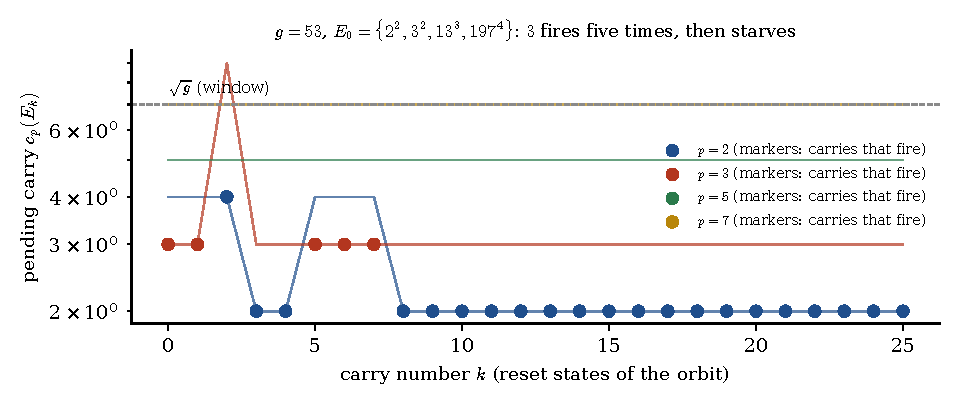
\includegraphics[width=0.97\linewidth]{figs/fig_competition.pdf}
\caption{Prime-carry competition in an actual orbit at \(g=53\) (seed exponents \(\{2{:}2,\,3{:}2,\,13{:}3,\,197{:}4\}\), first sixteen steps cross-checked against direct iteration of \(C\)). The scheduler (Theorem~\ref{thm:scheduler}) lets the prime with the smallest pending carry fire: the prime \(3\) fires five times during the transient, interleaved with \(2\), and then starves, after which the prime \(2\) carries alone, exactly as Theorem~\ref{thm:dominance} and Corollary~\ref{cor:starve} require.}\label{fig:competition}
\end{figure}

\section{Consequences}

\begin{theorem}[The scaling factor is a prime power]\rec{F.T61}\scope{C}\label{thm:rho}
Let \(p\) be the active prime (Theorem~\ref{thm:dominance}), \(s\) the minimal translation period of \(\Abs_p\subseteq\Z/o_p\) (the least \(s\mid o_p\) with \(\Abs_p+s=\Abs_p\)), and \(j_1,\dots,j_m\) the gaps of \(\Abs_p\) inside one period, \(\sum_ij_i=s\). Then the eventual orbit has \(\gamma\)-period
\[
P_\gamma=\sum_{i=1}^m\big(p^{2j_i}-1\big),\qquad L_{n+P_\gamma}=p^sL_n,\qquad x_{n+P_\gamma}=p^{2s}x_n.
\]
So \(\rho=p^s\) is a prime power. For \(G_\infty=1\): \(p=2\), \(s=1\), \(P_\gamma=3\), \(\rho=2\). Every orbit of the collective map therefore eventually satisfies \(x_{n+P}=p^{2s}x_n\) with \(p\) prime.
\end{theorem}
\begin{proof}
One active prime: the carries are the successive gaps of \(\Abs_p\) around \(\Z/o_p\) (Theorem~\ref{thm:odometer}), with cycle lengths \(p^{2j}-1\) (Theorem~\ref{thm:carrycomp}). The carry word is periodic with minimal rotation period equal to the minimal translation period \(s\) of \(\Abs_p\) (its gap sequence repeats exactly when \(\Abs_p\) is invariant under the translation), and over that period \(e_p\) increases by \(\sum_ij_i=s\) while all other exponents are constant. The \(\gamma\)-sequence is determined by the carry word, so it is periodic with period \(P_\gamma\), and \(L_{n+P_\gamma}=p^sL_n\); then \(x_{n+P_\gamma}=\gamma L_{n+P_\gamma}^2/g=p^{2s}x_n\).
\end{proof}

(The class period of Theorem~\ref{thm:closure} may be a multiple \(o_p/s\) of \(P_\gamma\), because the class records \(e_p\bmod o_p\) while the carry word only sees it through \(\Abs_p\).) Examples: \(g=31\): \(\Abs=\{0,2,4\}\bmod5\), \(s=5\), \(\rho=32\), \(P_\gamma=15+15+3=33\); \(g=17\): \(s=8\), \(\rho=256\); \(g=11,31,367\) with \(\Abs=\Z/o_p\): \(s=1\), \(\rho=q\).

\begin{corollary}[Logarithmic reach for every orbit]\label{cor:logreach}
For every orbit of \(C\), the set \(U\) of all moduli \(d\) that ever occur in a fibre satisfies \(U(X)=\#\{d\in U:d\le X\}=O(\log X)\), with a constant depending on the orbit.
\end{corollary}
\begin{proof}
If \(G_\infty=1\), Theorem~\ref{thm:L4} gives it. Otherwise the orbit is eventually persistent and, by Theorem~\ref{thm:dominance}, from some time \(n_0\) on \(L_n=c\,p^{e_n}\) with \(c\) constant, \(p\) the active prime and \(e_n\to\infty\). By monotonicity (Theorem~\ref{thm:mono}), every modulus ever occurring is either in the finite set \(\bigcup_{n\le n_0}\Dx(x_n)\) or divides \(cp^k\) for some \(k\); the second kind has the form \(d=ap^i\) with \(a\mid c\), and \(d\le X\) forces \(i\le\log_pX\). So \(U(X)\le|U_0|+\tau(c)(1+\log_2X)\).
\end{proof}
The \emph{unbounded multiplicity} of Chapter~\ref{ch:growth} (\(R(x_n)\to\infty\)) therefore coexists with \emph{extreme sparsity of the moduli} that generate it: each orbit reaches only logarithmically many indices, all of the shape \(a\,p^i\).

\begin{figure}[t]
\centering
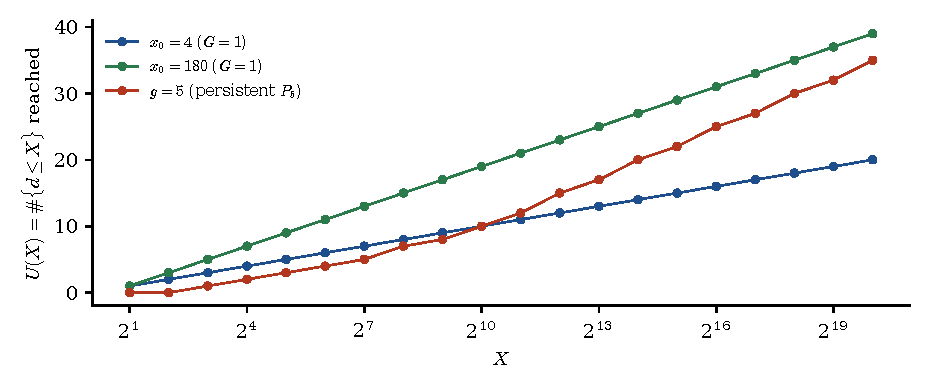
\includegraphics[width=0.9\linewidth]{figs/fig_reach.pdf}
\caption{Reach counting \(U(X)=\#\{d\le X\}\) for three orbits (75 exact steps each): two orbits at \(G=1\) (\(x_0=4\) and \(x_0=180\)) and the persistent orbit at \(g=5\) of Theorem~\ref{thm:T42}. The growth is logarithmic in \(X\), as Corollary~\ref{cor:logreach} asserts, even though the fibre multiplicity \(R(x_n)\) is unbounded.}\label{fig:reach}
\end{figure}

\begin{theorem}[Coprime clocks]\rec{F.T62}\scope{C}\label{thm:coprime}
Let \(g\) be an odd prime and \(p\ne q\) saturated primes with orders \(o_p,o_q\) and background \(F\) (the residues of the frozen part). Then \(\mathcal A_{-p}=\langle q\rangle F\) is a union of cosets of \(\langle q\rangle\) and \(\Abs_p=\{k:p^{-k}\in\langle q\rangle F\}\) is invariant under \(k\mapsto k+\tau_p\), \(\tau_p=o_p/\gcd(o_p,o_q)\); likewise \(\Abs_q\) is \(\tau_q\)-periodic with \(\tau_q=o_q/\gcd(o_p,o_q)\). The numbers \(\tau_p\) and \(\tau_q\) are coprime.
\end{theorem}
\begin{proof}
\((\Z/g)^\times\) is cyclic, so \(|\langle p\rangle\cap\langle q\rangle|=\gcd(o_p,o_q)\), and \(p^\tau\in\langle q\rangle\) iff \(\tau\) is a multiple of \(o_p/\gcd(o_p,o_q)\). Then \(p^{-(k+\tau_p)}\in\langle q\rangle F\iff p^{-k}\in\langle q\rangle F\). The numbers \(o_p/\gcd(o_p,o_q)\) and \(o_q/\gcd(o_p,o_q)\) are coprime.
\end{proof}

Two clocks can therefore be coupled only through the common background \(F\), and their natural periods share no factor, so phase locking is excluded by the arithmetic as well; Theorem~\ref{thm:dominance} shows that the absence of coupling is not even needed: the scheduler rule alone excludes coexistence.

\begin{remark}[Scope of the coexistence question]\rec{F.T63}\scope{C}\label{rem:T63}
The ``threshold-overlap'' lemma (if \(p,q\) both occur infinitely often then \(B_p^+>B_q^-\) and \(B_q^+>B_p^-\)) is true and is sharpened by Theorem~\ref{thm:dominance} to the contradictory pair \(m_q>m_p\), \(m_p>m_q\). In particular no pair of counter-rotating odometers with alternating carry thresholds exists, even in the abstract system: with the minimum-rule scheduler the odometer with the larger worst-case pending carry is always the one that stops. Every candidate pair of coexisting primes is excluded by proof, not by search. The proof of Theorem~\ref{thm:dominance} does not use primality of \(g\), so the statement covers even and composite moduli as well; the numerical sample behind the examples is almost entirely prime \(g\).
\end{remark}
